\documentclass[xcolor=dvipsnames]{beamer}
\usepackage{multicol}
\usepackage{xy}
\everymath{\displaystyle}
\mode<presentation>
{\usetheme{Warsaw}\setbeamercovered{dynamic}}
\usecolortheme{crane}
\usepackage{beamerfoils}
\pgfdeclareimage[height=1in]{university-logo}{ISULogo}
\logo{\pgfuseimage{university-logo}}
\setbeamertemplate{navigation symbols}{}
\title[Syllabus highlights]{Math 104\\Syllabus highlights}
\author{Dr Marcus Bishop}
\subject{Math 104}
\beamerdefaultoverlayspecification{<+->}
\theoremstyle{definition}
\newtheorem{remark}{Remark}
\newtheorem{impact}{Impact}
\newtheorem{situation}{Situation}
\newtheorem{question}{Question}
\usepackage{arev}
\usepackage{tensor}
\newcommand\npr[2]{\tensor[_{#1}]P{_{#2}}}
\newcommand\ncr[2]{\tensor[_{#1}]C{_{#2}}}
\usepackage{cancel}
\newcommand{\hs}{\alert{\varheart}}
\newcommand{\ds}{\alert{\vardiamond}}
\newcommand{\s}{\spadesuit}
\newcommand{\cs}{\clubsuit}
\begin{document}
\begin{frame}\titlepage\end{frame}
\LogoOff

\begin{frame}{Instructor and TA contact information}
\begin{itemize}
\item Full syllabus available on
\href{https://bb.its.iastate.edu}{\color{blue} Blackboard}
\item This document and all slides presented in class
available on
\href{https://bb.its.iastate.edu}{\color{blue} Blackboard}
\item Blue words hyperlinks
\item Instructor's office hours:
9:00--12:00 Tuesdays and Thursdays in Carver~418
\item \dots or by special arrangement
\item Graduate assistant for course is
\href{mailto:mws@iastate.edu}{\color{blue} Minwoo Shin}
\item Minwoo's office hours:
12:00--14:00 Mondays and Wednesdays in Carver 244
\end{itemize}
\end{frame}

\begin{frame}{Flowchart for resolving problems}
\begin{enumerate}
\item Consult the FAQ on
\href{https://bb.its.iastate.edu}{\color{blue} Blackboard}
\item Consult the syllabus on
\href{https://bb.its.iastate.edu}{\color{blue} Blackboard}
\item Email or visit \href{mailto:mws@iastate.edu}{\color{blue}Minwoo}
if question involves
\begin{itemize}
\item Missing homework assignments
\item Early homework submission
\item Scores incorrectly entered into
\href{https://bb.its.iastate.edu}{\color{blue} Blackboard}
\end{itemize}
\item Email or visit \href{mailto:mbishop@iastate.edu}{\color{blue}the instructor}
for all other questions
\end{enumerate}
\end{frame}

\begin{frame}{Online exercises}
\begin{itemize}
\item Online exercises delivered through
\href{http://iastate.mylabsplus.com}{\color{blue} MyLabsPlus}
\item Subscription comes with textbook
\item Can also be purchased separately
\item Assignments always due at 10:00 AM
\item 
\href{http://iastate.mylabsplus.com}{\color{blue}ML+}
assignments usually due Mondays and Wednesdays
\item Written assignments due in class Fridays (see below)
\item Run Browser Checker
\item Complete Assignment Zero to orient yourself (not required)
\item Contact
\href{mailto://mathmlp@iastate.edu}{\color{blue}\tt mathmlp@iastate.edu}
in case of problems
\end{itemize}
\end{frame}

\begin{frame}{Caution}
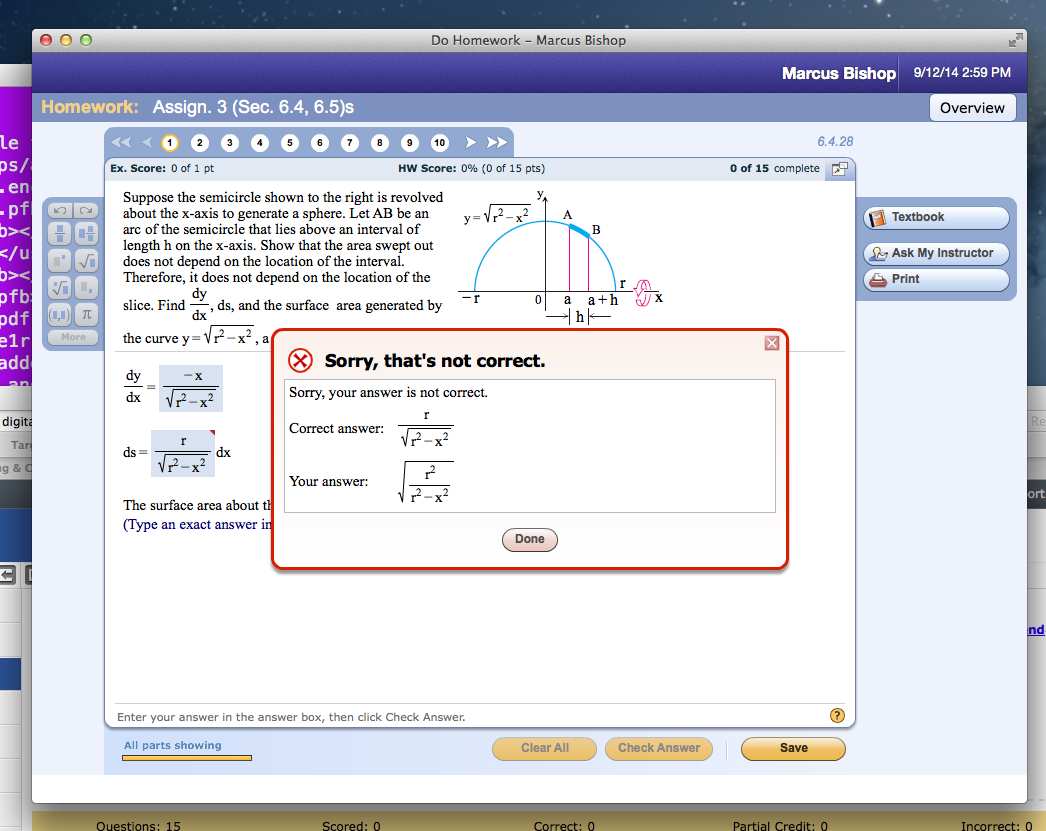
\includegraphics[scale=.4]{MLPError}
\end{frame}

\begin{frame}{Written assignments}
\begin{itemize}
\item Written assignments posted on
\href{https://bb.its.iastate.edu}{\color{blue} Blackboard}
\item Written assignments collected \alert{every Friday}
at \alert{beginning} of class
\item \dots except first and last weeks of class
\item Might occasionally assign written assignments
due Mondays and Wednesdays
\item Written assignments more difficult than 
\href{http://iastate.mylabsplus.com}{\color{blue}ML+}
and cover material not available in
\href{http://iastate.mylabsplus.com}{\color{blue}ML+}
\end{itemize}
\end{frame}

\begin{frame}{Written assignment submission}
\begin{itemize}
\item Can submit written assignments early in Minwoo's office
\item Please don't
\begin{itemize}
\item slide homework under office doors
\item try to submit to instructor in class
\item email homework to Minwoo
\end{itemize}
\item Written assignments can \alert{never} be accepted late,
since we discuss answers in class after collecting
\item You must arrive on time to submit homework
\item However, we drop three lowest written assignment scores from final grade
\end{itemize}
\end{frame}

\begin{frame}{Quiz and exam dates}
\begin{center}\begin{tabular}{rrl}
Quiz 1:&21&January\\
Exam 1:&4&February\\
Quiz 2:&18&February\\
Exam 2:&4&March\\
Quiz 3:&25&March\\
Exam 3:&8&April\\
Quiz 4:&22&April
\end{tabular}\end{center}
\begin{itemize}
\item Mark all of these events on your calendar
\item Quizzes and exams can \alert{never} be rescheduled
except in cases of death, severe illness, military service,
school-sponsored trip, or jury duty
\item Rescheduling requires documentation
\end{itemize}
\end{frame}

\begin{frame}{Calculation of final grades}
\begin{itemize}
\item Course not ``curved''
\item Grades calculated by formula
\[\frac{450e}{300}+\frac{100w}{10W}
+\frac{100m}{M}+\frac{150q}{40}+\frac{200f}{40}\]
\item $e$ the sum of exam scores
\item $w$ the sum of written assignment scores
\item $W$ the number of written assignments
\item $m$ the sum of
\href{http://iastate.mylabsplus.com}{\color{blue}ML+} scores
\item $M$ the number of points possible in
\href{http://iastate.mylabsplus.com}{\color{blue}ML+}
\item $q$ the sum of quiz scores
\item $f$ the final exam score
\end{itemize}
\end{frame}

\begin{frame}{Grade ranges}
\begin{itemize}
\item Grand total calculated by formula above, out of 1000
\item Grades assigned according to schedule below
\begin{center}\begin{tabular}{rr}
A&850--1000\\
B&750--849\\
C&650--749\\
D&550--649\\
F&0--449
\end{tabular}\end{center}
\end{itemize}
\end{frame}

\end{document}
